\documentclass[12pt]{article}

\usepackage[hidelinks]{hyperref}
\usepackage[margin=0.5in]{geometry}
\usepackage{tikz}

% Commands
\newcommand{\definition}[1]{\textbf{\underline{DEFINITION:}}{ #1}}
\newcommand{\braces}[1]{\{#1\}}


\title{Lecture 1, MATH 239 - Introduction to Combinatorics\\ Graph Theory 1 - Graph, Vertex, Edge, Complete Graph, Path, Cycle, Complete Bipartite Graph}
\date{January 4, 2017}
\author{Professor Luke Postle\\ Notes by Dadi Zhang (\href{http://www.dzed.me}{dzed.me}) \\ Faculty of Mathematics, University of Waterloo}
\begin{document}

\maketitle

\definition{A \textbf{graph} is a set of elements called \textbf{vertices} and a set of pairs of distinct vertices called \textbf{edges}. If $G$ is a graph, we let $V(G)$ denote the set of vertices and $E(G)$ denote the set of edges.} \\

We tend to draw graphs where vertices are points and edges are lines/curves connecting the pairs of vertices.

\textbf{Example:} $V = \left\{a\right\}, E = \emptyset$ \hspace{10px}
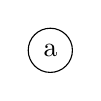
\begin{tikzpicture}
	\node[shape=circle, draw=black]{a};
\end{tikzpicture} \\

\textbf{Example:} $V = \left\{x, y, z\right\}, E = \left\{xy, yz\right\}$ \hspace{10px}
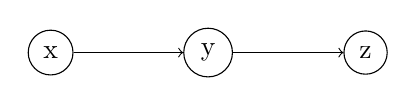
\begin{tikzpicture}
	\node[shape=circle, draw=black](x) at (0, 0){x};
	\node[shape=circle, draw=black](y) at (2, 0){y};
	\node[shape=circle, draw=black](z) at (4, 0){z};
	
	\path [->](x) edge (y);
	\path [->](y) edge (z);
\end{tikzpicture} \\

\textbf{Example:} $V = \emptyset, E = \emptyset$ known as the empty graph.

\textbf{Example:} $V = \left\{1, 2, 3, 4, 5\right\}, E = \left\{12, 34, 35, 45\right\}$ \hspace{10px}
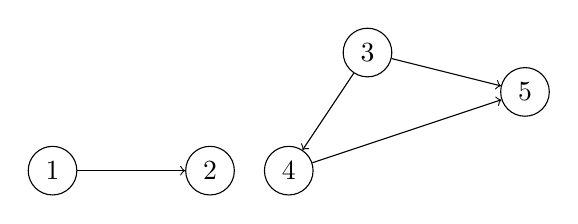
\begin{tikzpicture}
	\node[shape=circle, draw=black](1) at (0, 0){1};
	\node[shape=circle, draw=black](2) at (2, 0){2};
	\node[shape=circle, draw=black](3) at (4, 1.5){3};
	\node[shape=circle, draw=black](4) at (3, 0){4};
	\node[shape=circle, draw=black](5) at (6, 1){5};
	
	\path [->](1) edge (2);
	\path [->](3) edge (4);
	\path [->](3) edge (5);
	\path [->](4) edge (5);
\end{tikzpicture} \\
\vspace{10px}

\definition{$K_n$ denotes the complete graph on n vertices where complete means all pairs of vertices are edges.}

\textbf{Example:}
$K_3$
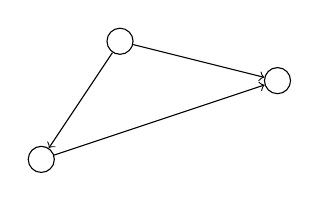
\begin{tikzpicture}
	\node[shape=circle, draw=black](3) at (4, 1.5){};
	\node[shape=circle, draw=black](4) at (3, 0){};
	\node[shape=circle, draw=black](5) at (6, 1){};
	
	\path [->](3) edge (4);
	\path [->](3) edge (5);
	\path [->](4) edge (5);
\end{tikzpicture} \hspace{20px}
$K_4$
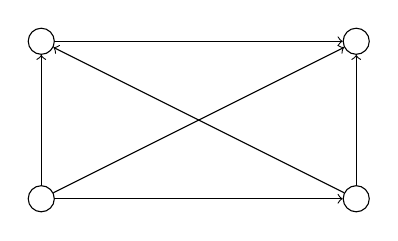
\begin{tikzpicture}
	\node[shape=circle, draw=black](3) at (0, 0){};
	\node[shape=circle, draw=black](4) at (4, 0){};
	\node[shape=circle, draw=black](5) at (0, 2){};
	\node[shape=circle, draw=black](6) at (4, 2){};
	
	\path [->](3) edge (4);
	\path [->](3) edge (5);
	\path [->](3) edge (6);
	\path [->](4) edge (5);
	\path [->](4) edge (6);
	\path [->](5) edge (6);
\end{tikzpicture} \\

\definition{$C_n$ denotes the cycle on n vertices. $P_n$ denotes the path (or path graph) on n vertices.} \\

\definition{$K_{m,n}$ denotes a \textbf{complete bipartite graph} on m and n vertices. A complete bipartite graph is a special kind of bipartite graph where every vertex of the first set is connected to every vertex of the second set. $V = \braces{x_1, x_2,..., x_m, y_1, y_2,..., y_n}$} \\

\textbf{Example:} 
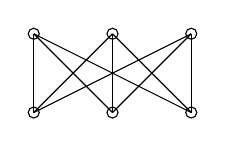
\begin{tikzpicture}[]
\foreach \x in {0,1,2}
\foreach \y in {0,1,2}
{\draw (\y,0) -- (\x,1);}
\foreach \x in {0,1,2}{
\draw (\x,0) circle (2pt);
\draw (\x,1) circle (2pt);}
\end{tikzpicture}



\end{document}